\begin{frame}{Lexical Search: Inverted Index and BM25}
  \begin{itemize}\footnotesize
    \item[\textcolor{red}{$\blacktriangleright$}] \textbf{BM25} scores document $d$ for query $q$ by adding one weight per query term $t$:
      \[ \text{BM25}(q,d) = \sum_{t \in q} \log\frac{N - n_t + 0.5}{n_t + 0.5} \cdot \frac{tf_{t,d}}{tf_{t,d} + k_1\,(1 - b + b\, dl/avdl)} \]
      {\scriptsize $N$: documents in the collection; $n_t$: those containing $t$; $tf_{t,d}$: count of $t$ in $d$; $dl$, $avdl$: length of $d$ and mean length; $k_1$, $b$: constants.}
  \end{itemize}
  \begin{columns}[T,onlytextwidth]
    \column{0.55\textwidth}
      \begin{itemize}\footnotesize\itemsep0.3em
        \item[\textcolor{red}{$\blacktriangleright$}] \textbf{Inverted index:} each term points to a posting list, the documents that contain it with a count each. A query reads only its own terms' lists, so documents sharing no term are never scored.
        \item[\textcolor{red}{$\blacktriangleright$}] The log factor is the \textbf{IDF} (inverse document frequency) weight, as in TF-IDF (covered earlier). The $tf$ factor saturates: ``any one term's contribution to the document score cannot exceed a saturation point''. $k_1$ sets how fast, $b \in [0,1]$ how much long documents are discounted; $1.2 < k_1 < 2$ and $0.5 < b < 0.8$ suit many collections.
      \end{itemize}
    \column{0.43\textwidth}
      {\centering
      \resizebox{\linewidth}{!}{%
      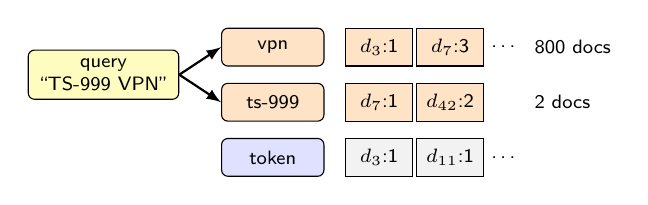
\begin{tikzpicture}[font=\sffamily\scriptsize, >=latex,
          term/.style={draw, rounded corners=0.08cm, fill=blue!12, minimum width=1.3cm, minimum height=0.48cm},
          post/.style={draw, fill=gray!10, minimum width=0.85cm, minimum height=0.48cm, inner sep=1pt},
          hot/.style={draw, fill=orange!22, minimum width=0.85cm, minimum height=0.48cm, inner sep=1pt}]
        \node[term, fill=orange!22] (vpn) at (0,1.4) {vpn};
        \node[hot] at (1.35,1.4) {$d_3$:1};
        \node[hot] at (2.25,1.4) {$d_7$:3};
        \node at (2.95,1.4) {\dots};
        \node[anchor=west] at (3.2,1.4) {800 docs};
        \node[term, fill=orange!22] (ts) at (0,0.7) {ts-999};
        \node[hot] at (1.35,0.7) {$d_7$:1};
        \node[hot] at (2.25,0.7) {$d_{42}$:2};
        \node[anchor=west] at (3.2,0.7) {2 docs};
        \node[term] at (0,0) {token};
        \node[post] at (1.35,0) {$d_3$:1};
        \node[post] at (2.25,0) {$d_{11}$:1};
        \node at (2.95,0) {\dots};
        \node[draw, rounded corners=0.08cm, fill=yellow!25, align=center] (q) at (-2.15,1.05) {query\\``TS-999 VPN''};
        \draw[->, thick] (q.east) -- (vpn.west);
        \draw[->, thick] (q.east) -- (ts.west);
      \end{tikzpicture}}\\[0.25em]
      {\scriptsize Part of an index over $N = 10{,}000$ documents (document:count). The rare code gets IDF 8.3, vpn 2.4 (natural log): exact identifiers are where BM25 is strongest.\par}\par}
      \begin{itemize}\scriptsize
        \item[\textcolor{red}{$\blacktriangleright$}] \textbf{Weakness, vocabulary mismatch:} a query and a passage that name one thing with different words (``bad guy'', ``villain'') share no term.
      \end{itemize}
  \end{columns}
  \vspace{0.1em}
  {\scriptsize Robertson and Zaragoza, ``The Probabilistic Relevance Framework: BM25 and Beyond,'' \textit{Foundations and Trends in Information Retrieval} 3(4), 2009, \href{https://doi.org/10.1561/1500000019}{doi:10.1561/1500000019}, Eqs.~3.3 and 3.15, Sections~2.4, 3.4.2 and 3.5.\par}
\end{frame}

\begin{frame}{Dense Retrieval with a Bi-Encoder: DPR}
  \begin{columns}[T,onlytextwidth]
    \column{0.52\textwidth}
      \begin{itemize}\footnotesize\itemsep0.3em
        \item[\textcolor{red}{$\blacktriangleright$}] \textbf{Bi-encoder:} a dual encoder (covered earlier) for text: question and passage are embedded separately and compared by a dot product. DPR (dense passage retriever) uses two BERT-base encoders and their [CLS] vectors, $d = 768$:
          \[ \text{sim}(q,p) = E_Q(q)^{\top} E_P(p) \]
          {\scriptsize $E_Q$, $E_P$: question and passage encoders.}
        \item[\textcolor{red}{$\blacktriangleright$}] \textbf{Dense retrieval:} passages are embedded once, offline, into an approximate nearest-neighbour (ANN) index (covered in the CV course). ``Bad guy'' can now find ``the villain Sauron''.
        \item[\textcolor{red}{$\blacktriangleright$}] \textbf{Training:} the contrastive softmax (covered in the CV course) with in-batch negatives, the batch's other gold passages, plus one hard negative per question: a top BM25 passage without the answer. It lifts top-20 accuracy from 70.8 to 77.3 (NQ dev, batch 32).
      \end{itemize}
    \column{0.46\textwidth}
      {\centering
      % Columns 1-4 hold the batch's gold passages, columns 5-8 one BM25 hard negative per question.
      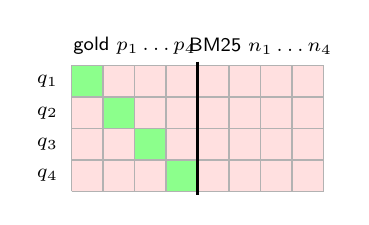
\begin{tikzpicture}[font=\sffamily\scriptsize]
        \foreach \row in {1,...,4} {
          \foreach \col in {1,...,8} {
            \ifnum\row=\col\relax
              \fill[green!45] ({(\col-1)*0.4},{-\row*0.4}) rectangle ++(0.4,0.4);
            \else
              \fill[red!12] ({(\col-1)*0.4},{-\row*0.4}) rectangle ++(0.4,0.4);
            \fi
          }
          \node[anchor=east] at (-0.05,{-\row*0.4+0.2}) {$q_{\row}$};
        }
        \draw[gray!60] (0,-1.6) grid[step=0.4] (3.2,0);
        \draw[thick] (1.6,0.05) -- (1.6,-1.65);
        \node[anchor=south] at (0.8,0.02) {gold $p_1 \dots p_4$};
        \node[anchor=south] at (2.4,0.02) {BM25 $n_1 \dots n_4$};
      \end{tikzpicture}\\[0.2em]
      {\scriptsize One batch, $B = 4$ (DPR: 128). Each row is a softmax with one positive (green) and $2B - 1$ negatives.\par}\vspace{0.4em}
      {\scriptsize
      \begin{tabular}{lcc}
        \toprule
        Natural Questions (NQ) test & top-20 & top-100 \\
        \midrule
        BM25 & 59.1 & 73.7 \\
        DPR & 78.4 & 85.4 \\
        \bottomrule
      \end{tabular}\par}\par}
      \vspace{0.2em}
      \begin{itemize}\scriptsize\itemsep0.2em
        \item[\textcolor{red}{$\blacktriangleright$}] Top-$k$ accuracy: share of questions answered by a passage in the top $k$.
        \item[\textcolor{red}{$\blacktriangleright$}] \textbf{Cost moves offline:} 995 questions/s at query time, against 23.7 per CPU thread for BM25 (Lucene); but embedding 21M passages took 8.8\,h on 8 GPUs plus 8.5\,h of indexing.
      \end{itemize}
  \end{columns}
  \vspace{0.1em}
  {\scriptsize Karpukhin et al., ``Dense Passage Retrieval for Open-Domain Question Answering,'' EMNLP 2020, \href{https://arxiv.org/abs/2004.04906v3}{arXiv:2004.04906v3}, Sections~1--3, 5.4, Tables~2--3.}
\end{frame}

\begin{frame}{Rerankers: Cross-Encoders over a Shortlist}
  \centering
  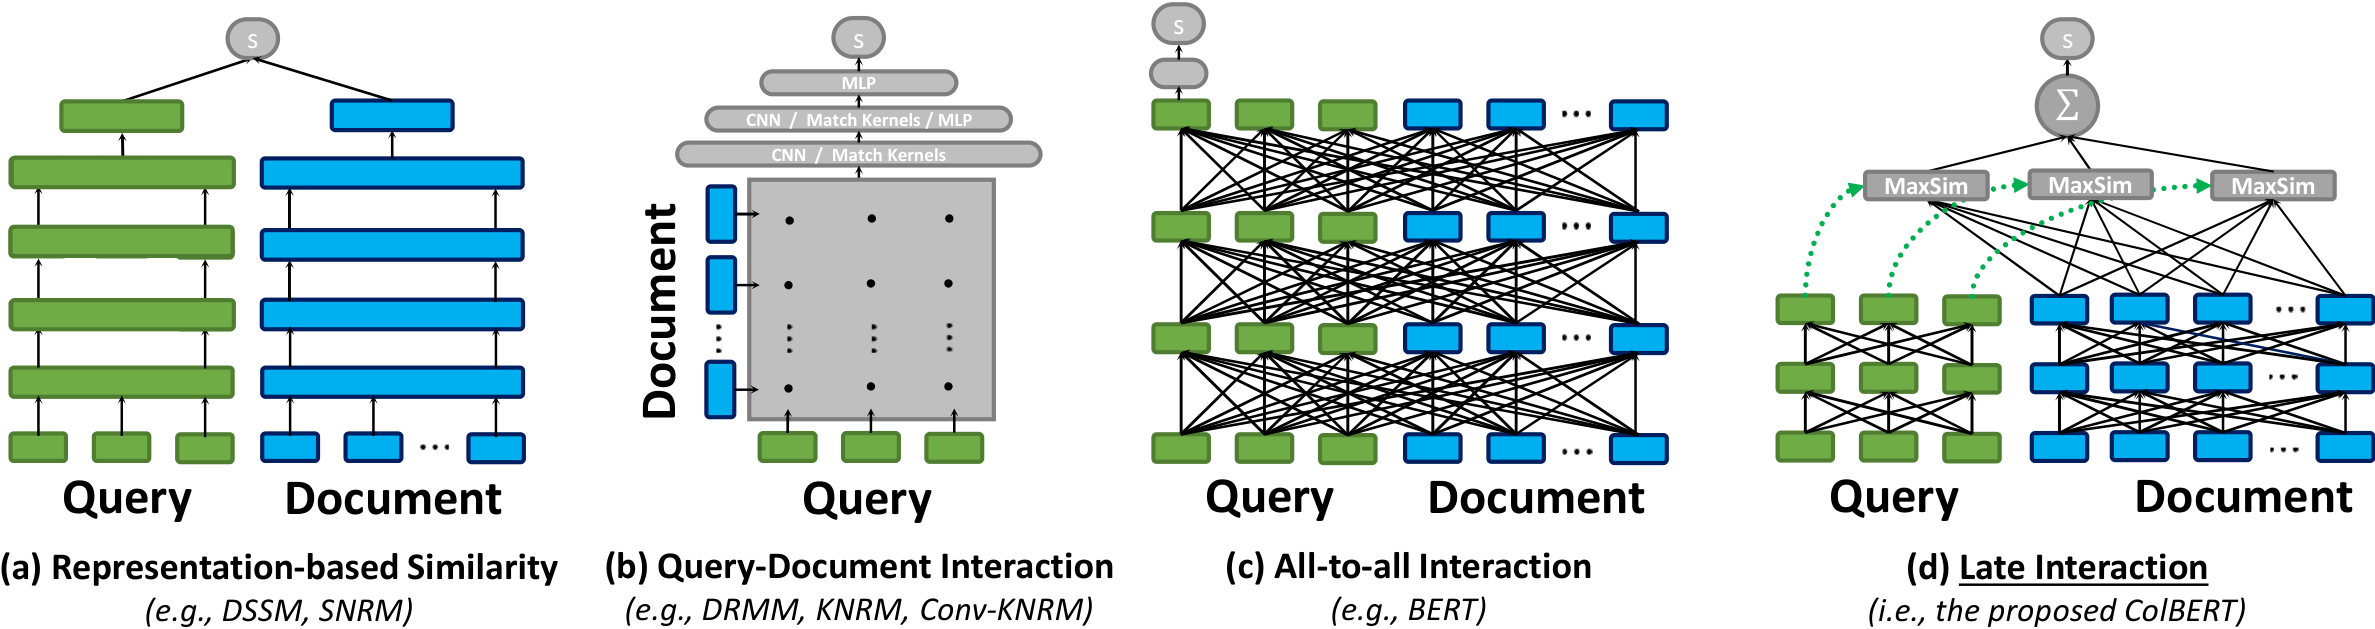
\includegraphics[width=\textwidth,height=0.33\textheight,keepaspectratio]{images/nlp-security-enterprise/colbert_fig2_matching_paradigms.png}\\[0.2em]
  {\scriptsize Khattab and Zaharia, ``ColBERT: Efficient and Effective Passage Search via Contextualized Late Interaction over BERT,'' SIGIR 2020, \href{https://arxiv.org/abs/2004.12832v2}{arXiv:2004.12832v2}, Figure~2.\par}
  \vspace{0.3em}
  \begin{columns}[T,onlytextwidth]
    \column{0.49\textwidth}
      \begin{itemize}\scriptsize\itemsep0.3em
        \item[\textcolor{red}{$\blacktriangleright$}] Panel (a) is the bi-encoder of the previous slide. A \textbf{cross-encoder}, panel (c), reads query and passage together, so every query token attends to every passage token. Nothing can be precomputed, so it only rescores a shortlist: it is a \textbf{reranker}.
        \item[\textcolor{red}{$\blacktriangleright$}] \textbf{monoBERT:} BERT-large on the concatenated pair; a layer on [CLS] gives the probability of relevance. Reranking BM25's top 1{,}000 on MS MARCO raised MRR@10 from 16.7 to 36.5.
      \end{itemize}
    \column{0.49\textwidth}
      \begin{itemize}\scriptsize\itemsep0.3em
        \item[\textcolor{red}{$\blacktriangleright$}] \textbf{Cost:} one forward pass per candidate: 10.7\,s per query for 1{,}000 passages with BERT-base, 32.9\,s with BERT-large (V100 GPU). Shortlists stay short: BEIR (two slides on) reranks BM25's top 100.
        \item[\textcolor{red}{$\blacktriangleright$}] \textbf{Retrieve, then rerank} (two-stage retrieval, covered in the CV course): tune the first stage (BM25, a bi-encoder, or both) for recall over 100 to 1{,}000 candidates, and the reranker for precision in the few chunks that reach the LLM.
      \end{itemize}
  \end{columns}
  \vspace{0.1em}
  {\scriptsize Nogueira and Cho, ``Passage Re-ranking with BERT,'' \href{https://arxiv.org/abs/1901.04085v5}{arXiv:1901.04085v5}, Table~1 (named monoBERT in Nogueira et al., \href{https://arxiv.org/abs/1910.14424v1}{arXiv:1910.14424v1}); latencies from the ColBERT paper, Table~1.\par}
\end{frame}

\begin{frame}{Late Interaction: ColBERT and MaxSim}
  \begin{columns}[T,onlytextwidth]
    \column{0.53\textwidth}
      \begin{itemize}\footnotesize\itemsep0.3em
        \item[\textcolor{red}{$\blacktriangleright$}] \textbf{Late interaction}, panel (d): encode query and document separately, as a bi-encoder does, but keep one vector per token and compare only at scoring time. ColBERT: one BERT, 128-dimensional normalised outputs.
        \item[\textcolor{red}{$\blacktriangleright$}] \textbf{MaxSim} score:
          \[ S_{q,d} = \sum_{i=1}^{|E_q|} \max_{j = 1,\dots,|E_d|} E_{q_i} \cdot E_{d_j}^{\top} \]
          {\scriptsize $E_q$: query token vectors, padded with [mask] to 32; $E_d$: document token vectors. Each query token keeps its best match.}
        \item[\textcolor{red}{$\blacktriangleright$}] Documents are encoded offline: reranking BM25's top 1{,}000 takes 61\,ms against 10{,}700\,ms for a BERT-base cross-encoder, at MRR@10 34.9 against 34.7. ColPali (covered earlier) applies MaxSim to page images.
      \end{itemize}
    \column{0.45\textwidth}
      \centering
      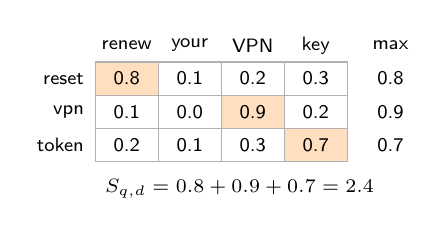
\begin{tikzpicture}[font=\sffamily\scriptsize,
          cell/.style={draw=gray!60, minimum width=0.8cm, minimum height=0.42cm, inner sep=0pt},
          best/.style={cell, fill=orange!25}]
        \node at (0.8,0.42) {renew};
        \node at (1.6,0.42) {your};
        \node at (2.4,0.42) {VPN};
        \node at (3.2,0.42) {key};
        \node at (4.15,0.42) {max};
        \node[anchor=east] at (0.38,0) {reset};
        \node[anchor=east] at (0.38,-0.42) {vpn};
        \node[anchor=east] at (0.38,-0.84) {token};
        \node[best] at (0.8,0) {0.8};     \node[cell] at (1.6,0) {0.1};     \node[cell] at (2.4,0) {0.2};     \node[cell] at (3.2,0) {0.3};
        \node[cell] at (0.8,-0.42) {0.1}; \node[cell] at (1.6,-0.42) {0.0}; \node[best] at (2.4,-0.42) {0.9}; \node[cell] at (3.2,-0.42) {0.2};
        \node[cell] at (0.8,-0.84) {0.2}; \node[cell] at (1.6,-0.84) {0.1}; \node[cell] at (2.4,-0.84) {0.3}; \node[best] at (3.2,-0.84) {0.7};
        \node at (4.15,0) {0.8};
        \node at (4.15,-0.42) {0.9};
        \node at (4.15,-0.84) {0.7};
        \node[anchor=west] at (0.4,-1.4) {$S_{q,d} = 0.8 + 0.9 + 0.7 = 2.4$};
      \end{tikzpicture}\\[0.2em]
      {\scriptsize Illustrative values: ``reset'' meets ``renew'' and ``token'' meets ``key'' with no shared word.\par}\vspace{0.4em}
      {\scriptsize
      \begin{tabular}{lr}
        \toprule
        MS MARCO index, 8.8M passages & size \\
        \midrule
        ColBERT, 128 dims, 32-bit & 286\,GiB \\
        ColBERT, 128 dims, 16-bit & 143\,GiB \\
        ColBERTv2, 1-bit residuals & 16\,GiB \\
        one 768-d 32-bit vector per passage & $\approx$25\,GiB \\
        \bottomrule
      \end{tabular}\par}
      \vspace{0.2em}
      {\scriptsize ColBERTv2 stores a token vector as its nearest centroid plus 1 bit per dimension: 20 bytes instead of 256.\par}
  \end{columns}
  \vspace{0.1em}
  {\scriptsize Khattab and Zaharia, \href{https://arxiv.org/abs/2004.12832v2}{arXiv:2004.12832v2}, Tables~1, 4; Santhanam et al., ``ColBERTv2,'' NAACL 2022, \href{https://arxiv.org/abs/2112.01488v3}{arXiv:2112.01488v3}, Sections~3.3, 5.3.\par}
\end{frame}

\begin{frame}{Zero-Shot Evidence and Hybrid Fusion}
  \begin{columns}[T,onlytextwidth]
    \column{0.52\textwidth}
      \begin{itemize}\scriptsize
        \item[\textcolor{red}{$\blacktriangleright$}] \textbf{BEIR:} 18 public datasets from 9 retrieval tasks (fact checking, question answering, argument retrieval, and more), used zero-shot: models trained on MS MARCO (DPR: on NQ and three other QA sets) are scored on unseen domains. nDCG@10 (covered earlier):
      \end{itemize}
      \vspace{0.2em}
      {\centering\scriptsize\setlength{\tabcolsep}{3pt}
      \begin{tabular}{lcccc}
        \toprule
        Dataset & BM25 & DPR & ColBERT & BM25+CE \\
        \midrule
        MS MARCO & 0.228 & 0.177 & 0.401$^{\ast}$ & 0.413$^{\ast}$ \\
        TREC-COVID & 0.656 & 0.332 & 0.677 & 0.757 \\
        BioASQ & 0.465 & 0.127 & 0.474 & 0.523 \\
        NQ & 0.329 & 0.474$^{\ast}$ & 0.524 & 0.533 \\
        FiQA-2018 & 0.236 & 0.112 & 0.317 & 0.347 \\
        Touch\'e-2020 & 0.367 & 0.131 & 0.202 & 0.271 \\
        \midrule
        Avg.\ vs BM25 & & $-47.7\%$ & $+2.5\%$ & $+11\%$ \\
        \bottomrule
      \end{tabular}\par}
      \vspace{0.2em}
      {\scriptsize $^{\ast}$ in-domain. BM25+CE: BM25's top 100 reranked by a MiniLM cross-encoder. Last row as printed in BEIR, which does not say how it averages.\par}
    \column{0.46\textwidth}
      \begin{itemize}\scriptsize\itemsep0.35em
        \item[\textcolor{red}{$\blacktriangleright$}] Out of domain, BM25 is hard to beat: bi-encoders fall below it under domain shift (BioASQ) and task shift (Touch\'e-2020). The reranker wins on 16 of 18 datasets, at 450\,ms per query (GPU, 1M documents) against 20\,ms for BM25 (CPU).
        \item[\textcolor{red}{$\blacktriangleright$}] \textbf{Hybrid search:} run BM25 and a dense retriever side by side and fuse by rank, since their scores sit on unrelated scales. \textbf{Reciprocal rank fusion (RRF):}
          \[ \text{RRF}(d) = \sum_{r \in R} \frac{1}{k + r(d)} \]
          $R$: the input rankings; $r(d)$: rank of $d$ in $r$, no term if absent; $k = 60$, set in a pilot, where the choice ``was not critical''.
        \item[\textcolor{red}{$\blacktriangleright$}] \textbf{Example:} first in BM25 and third in the dense list gives $1/61 + 1/63 = 0.0323$; second in one list only gives $1/62 = 0.0161$. In its pilot and TREC experiments, RRF beat the best single run and two other fusion methods by 4--5\% on average.
      \end{itemize}
  \end{columns}
  \vspace{0.1em}
  {\scriptsize Thakur et al.\ (BEIR), NeurIPS 2021 Datasets and Benchmarks, \href{https://arxiv.org/abs/2104.08663v4}{arXiv:2104.08663v4}, Tables~2--3; Cormack, Clarke and B\"uttcher, ``Reciprocal Rank Fusion outperforms Condorcet and individual Rank Learning Methods,'' SIGIR 2009, \href{https://doi.org/10.1145/1571941.1572114}{doi:10.1145/1571941.1572114}.\par}
\end{frame}

\begin{frame}{Embeddings and Vector Search at Scale}
  \begin{columns}[T,onlytextwidth]
    \column{0.50\textwidth}
      \begin{itemize}\scriptsize\itemsep0.35em
        \item[\textcolor{red}{$\blacktriangleright$}] \textbf{MTEB} (Massive Text Embedding Benchmark): 58 datasets, 112 languages, 8 task types; ``no particular text embedding method dominates across all tasks''. The model with the best English average (ST5-XXL) was not the best retriever (SGPT-5.8B-msmarco: nDCG@10 50.25 against 42.24). Choose on retrieval, then test on your own queries.
        \item[\textcolor{red}{$\blacktriangleright$}] \textbf{Matryoshka embeddings} (MRL): the training loss is summed over nested prefixes $z_{1:m}$ of the embedding, $m \in \{8, 16, \dots, d\}$, so every prefix is a usable embedding and a store can truncate vectors without re-encoding. On ImageNet-1K retrieval, a 16-dimension shortlist reranked at 2{,}048 dimensions matched full-size search, about 14$\times$ faster.
        \item[\textcolor{red}{$\blacktriangleright$}] ANN indexes (IVF, product quantization, HNSW) are covered in the CV course. Their \textbf{knob} is search breadth (graph candidates kept, IVF lists probed): wider search raises recall and latency together. Tune it on recall@$k$ measured after any filter.
      \end{itemize}
    \column{0.48\textwidth}
      {\centering
      {\scriptsize Memory for 100M chunks of 1{,}024 dimensions (bytes per vector; $1\,\text{GB} = 10^9$ bytes):}\\[0.2em]
      {\scriptsize
      \begin{tabular}{lrr}
        \toprule
        Storage & bytes & total \\
        \midrule
        float32 & 4{,}096 & 409.6\,GB \\
        int8 & 1{,}024 & 102.4\,GB \\
        float32, 256 dims (MRL) & 1{,}024 & 102.4\,GB \\
        int8, 256 dims (MRL) & 256 & 25.6\,GB \\
        1 bit per dimension & 128 & 12.8\,GB \\
        \bottomrule
      \end{tabular}\par}\par}
      \vspace{0.3em}
      \begin{itemize}\scriptsize
        \item[\textcolor{red}{$\blacktriangleright$}] \textbf{Filtered search:} nearest neighbours among only the vectors whose metadata pass a predicate: a tenant, a date range, or a group on the document's ACL (access control list). \textbf{Pre-filtering} scans every passing vector exactly; cost grows with how many pass. \textbf{Post-filtering} searches the index, then drops failures: if a fraction $s$ pass, it visits about $k/s$ results to keep $k$, more when they lie far from the query. Filter-aware graphs (ACORN) walk only the passing subgraph: 2--1{,}000$\times$ more queries per second at 0.9 recall.
      \end{itemize}
  \end{columns}
  \vspace{0.1em}
  {\scriptsize Muennighoff et al., ``MTEB: Massive Text Embedding Benchmark,'' EACL 2023, \href{https://aclanthology.org/2023.eacl-main.148/}{aclanthology.org/2023.eacl-main.148}. Kusupati et al., ``Matryoshka Representation Learning,'' NeurIPS 2022, \href{https://arxiv.org/abs/2205.13147v3}{arXiv:2205.13147v3}. Patel et al., ``ACORN: Performant and Predicate-Agnostic Search Over Vector Embeddings and Structured Data,'' 2024, \href{https://arxiv.org/abs/2403.04871v1}{arXiv:2403.04871v1}.}
\end{frame}
